\documentclass[11pt,a4paper,titlepage,dvipdfmx]{jarticle}
\usepackage{geometry}
\geometry{left=25truemm,right=25truemm,top=25truemm,bottom=37truemm}
\usepackage{ascmac}
\usepackage{multirow}
\usepackage{diagbox}
\usepackage[dvipdfmx]{graphicx}
\usepackage{float}
\usepackage{amsmath,amssymb}
\usepackage{listings,jlisting}
\usepackage{url}
\renewcommand{\lstlistingname}{プログラムリスト}
\renewcommand{\labelenumii}{\arabic{enumii}).}
\lstset{
  basicstyle={\ttfamily},
  identifierstyle={\small},
  commentstyle={\smallitshape},
  keywordstyle={\small\bfseries},
  ndkeywordstyle={\small},
  stringstyle={\small\ttfamily},
  frame={tb},
  breaklines=true,
  columns=[l]{fullflexible},
  numbers=left,
  xrightmargin=0zw,
  xleftmargin=3zw,
  numberstyle={\scriptsize},
  stepnumber=1,
  numbersep=1zw,
  lineskip=-0.5ex
}
\title{\huge{画像処理}}
\author{電子情報工学科5年 \\学籍番号:17404}
\date{提出日:2021年12月20日}

\begin{document}
  \maketitle

  \section{目的}
    本科目達成度の確認のため課題を提出する。
  \section{予備知識}
    本課題では用いる画像はすべてラスター形式の画像である。特に無圧縮のBMP形式を用いる。BMP形式ではヘッダと呼ばれるファイル自体の情報などが
    記載された部分がある。本課題では各ピクセルの画素値の情報のみが必要であるためヘッダを削除する必要がある。ヘッダを削除したファイルのINC形式として
    作成した変換プログラムによって画素値を変換する。その後取り除いたヘッダを追加することで既存の画像ビューアソフトによって閲覧することができる。
    図\ref{fig:flow}に一連の処理の流れを示す。
    \begin{figure}[H]
      \centering
      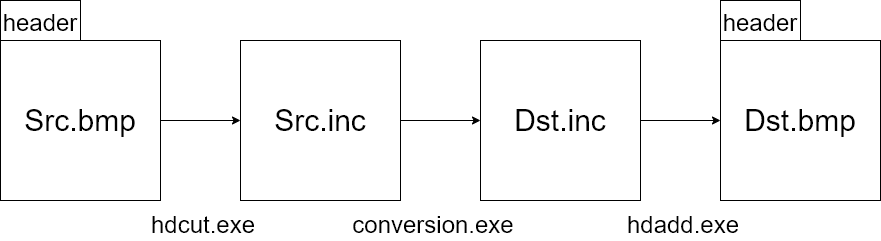
\includegraphics[scale=.4]{./flow.png}
      \caption{画像変換の処理}
      \label{fig:flow}
    \end{figure}
  \section{課題1(1)}
    本章では課題1(1)について課題内容、結果およびプログラムを示す。
    \subsection{課題内容}
      次に課題内容を示す.
      \begin{itembox}[l]{課題1(1)}
        画像処理のデータ変換において,次の変換の入力と出力の関係を表す各関数をグラフで表せ.
        \begin{enumerate}
          \item 輝度調整
          \item 等輝度線
        \end{enumerate}
      \end{itembox}
    \subsection{理論}
      本課題では入力画像としてグレースケール画像を用いる。そのため1ピクセルごとにその濃度値を何らかの関数によって変換する。
      式\eqref{eq:brightnessControl}に輝度調整の変換関数を示す。MAX,MINは指定する閾値である。
      \begin{equation} \label{eq:brightnessControl}
        f(x) = 
        \begin{cases}
        0   &   x < \text{MIN}  \\
        \frac{255(x - \text{MIN})}{\text{MAX} - \text{MIN}} & \text{MIN} \leqq x \leqq \text{MAX} \\
        255        &  x > \text{MAX} 
        \end{cases}
      \end{equation}
      式\eqref{eq:isohighlightLine}に等輝度線の変換関数を示す。RANGEはグレースケールで塗り分ける輝度幅である。
      \begin{equation} \label{eq:isohighlightLine}
        f(x) = 
        \begin{cases}
        x   &   \text{RANGE} \leqq 1  \\
        \frac{255 \cdot(x \% \text{RANGE})}{(\text{RANGE} - 1)} & else \\
        \end{cases}
      \end{equation}
    \subsection{結果}
      図\ref{fig:brightnessControl-graph}に輝度調整を行う変換関数を示す。また、図\ref{fig:isohighlightLine-graph}に等輝度線に変換する関数を示す。
      \begin{figure}[H]
        \centering
        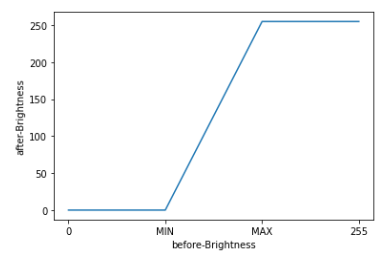
\includegraphics[scale=.8]{./brightnessControl.png}
        \caption{輝度調整}
        \label{fig:brightnessControl-graph}
      \end{figure} 
      \begin{figure}[H]
        \centering
        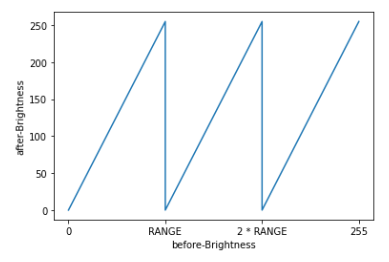
\includegraphics[scale=.8]{./isohighlightLine.png}
        \caption{等輝度線}
        \label{fig:isohighlightLine-graph}
      \end{figure} 
    \subsection{考察}
      図\ref{fig:brightnessControl-graph}より指定したMIN以下の濃度値では0に変換し、MAX以上である場合は濃度値を255に変換する。
      MINを超過し、MAX未満の濃度値は線形的に変換する。
      等輝度線では図\ref{fig:isohighlightLine-graph}のように指定したRANGE間隔で線形的に濃度値が上昇する。
  \section{課題1(2)}
    本章では課題1(2)について課題内容、結果およびプログラムを示す。
    \subsection{課題内容}
      次に課題内容を示す.
      \begin{itembox}[l]{課題1(2)}
        次の変換について元の画像と作成した画像の濃度値ヒストグラムを示せ.
        \begin{enumerate}
          \item 輝度調整
          \item 等輝度線
        \end{enumerate}
      \end{itembox}
    \subsection{結果}
      図\ref{fig:building-hist},\ref{fig:after-building-hist}にそれぞれ輝度調整を行う画像の濃度値ヒストグラム、輝度調整を行った画像の濃度値ヒストグラムを示す。MIN=75,MAX=170である。
      \begin{figure}[H]
        \centering
        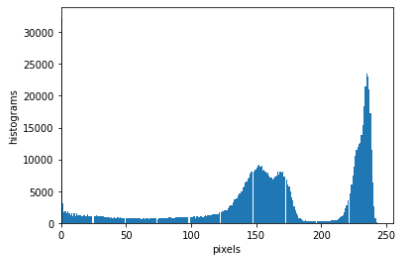
\includegraphics[scale=.8]{./building-hist.png}
        \caption{元画像の濃度値ヒストグラム}
        \label{fig:building-hist}
      \end{figure} 
      \begin{figure}[H]
        \centering
        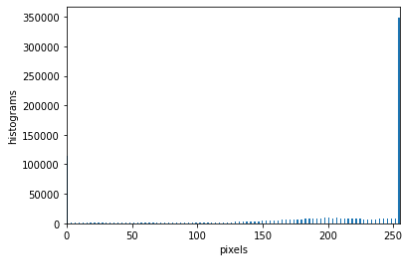
\includegraphics[scale=.8]{./after-building-hist.png}
        \caption{輝度調整後の画像の濃度値ヒストグラム}
        \label{fig:after-building-hist}
      \end{figure} 

      図\ref{fig:ham512-hist},\ref{fig:after-ham512-hist}にそれぞれ等輝度線に変換する画像の濃度値ヒストグラム、等輝度線画像の濃度値ヒストグラムを示す。RANGE=20である。
      \begin{figure}[H]
        \centering
        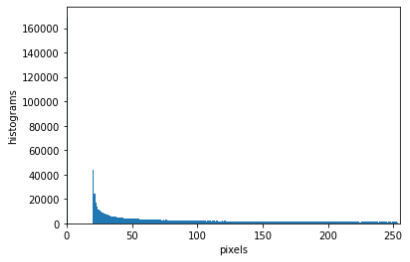
\includegraphics[scale=.8]{./ham512-hist.png}
        \caption{元画像の濃度値ヒストグラム}
        \label{fig:ham512-hist}
      \end{figure} 
      \begin{figure}[H]
        \centering
        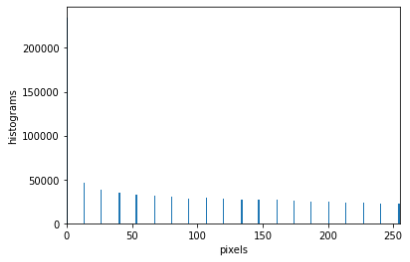
\includegraphics[scale=.8]{./after-ham512-hist.png}
        \caption{等輝度線画像の濃度値ヒストグラム}
        \label{fig:after-ham512-hist}
      \end{figure} 

    \subsection{考察}
      図\ref{fig:building-hist},\ref{fig:after-building-hist}より元画像では濃度値230程度の値が多いことがわかる。そのため輝度調整を行った画像の濃度値ヒストグラムでは255が一番多いことがわかる。
      図\ref{fig:after-ham512-hist}より等輝度線ではRANGEによって分割された濃度値のみが存在することがわかる。
  
  \section{課題1(3)}
  本章では課題1(3)について課題内容、結果およびプログラムを示す。
  \subsection{課題内容}
    次に課題内容を示す.
    \begin{itembox}[l]{課題1(3)}
      次の変換を行うプログラムを示せ.
      \begin{enumerate}
        \item 輝度調整
        \item 等輝度線
      \end{enumerate}
    \end{itembox}
  \subsection{プログラム}
    プログラムリスト\ref{p:brightnessControl}に輝度調整を行うプログラムを示す。
    \lstinputlisting[caption=輝度調整,label=p:brightnessControl]{../brightnessControl.c}

    コマンドライン引数として入出力ファイル、閾値となるmin,maxを指定する。getc関数によって入力バッファから1バイトずつ読み取りint型変数cに格納する。
    putc関数により出力バッファに書き込む。このとき式\eqref{eq:brightnessControl}を基に三項演算子によって場合分けを行う。

    プログラムリスト\ref{p:isohighlightLine}に等輝度線を出力するプログラムを示す。
    \lstinputlisting[caption=等輝度線,label=p:isohighlightLine]{../isohighlightLine.c}

    コマンドライン引数として入出力ファイル、輝度幅となるrangeを指定する。getc関数によって入力バッファから1バイトずつ読み取りint型変数cに格納する。
    putc関数により出力バッファに書き込む。このとき式\eqref{eq:brightnessControl}を基に変換を行う。

  \subsection{結果}
    図\ref{fig:building},\ref{fig:after-building}にそれぞれ輝度調整を行う画像、輝度調整を行った画像を示す。MIN=75,MAX=170である。

    \begin{figure}[H]
      \centering
      \includegraphics[scale=.8]{./building.bmp}
      \caption{元画像}
      \label{fig:building}
    \end{figure} 
    \begin{figure}[H]
      \centering
      \includegraphics[scale=.8]{./after-building.bmp}
      \caption{輝度調整後の画像}
      \label{fig:after-building}
    \end{figure} 

    図\ref{fig:ham512},\ref{fig:after-ham512}にそれぞれ等輝度線に変換する画像、等輝度線画像を示す。RANGE=20である。

    \begin{figure}[H]
      \centering
      \includegraphics[scale=.8]{./ham512.bmp}
      \caption{元画像}
      \label{fig:ham512}
    \end{figure} 
    \begin{figure}[H]
      \centering
      \includegraphics[scale=.8]{./after-ham512.bmp}
      \caption{等輝度線画像}
      \label{fig:after-ham512}
    \end{figure} 

  \subsection{考察}
    図\ref{fig:building},\ref{fig:after-building}より元画像の空の部分は白く、木の部分は黒くなっていることがわかる。従って輝度調整ができていると言える。

\section{課題2(1)}
  本章では課題2(1)について課題内容、結果およびプログラムを示す。
  \subsection{課題内容}
    次に課題内容を示す.
    \begin{itembox}[l]{課題2(1)}
      3$\times$3空間フィルタによる8近傍ラプラシアンを実行し,エッジ抽出を行え.
    \end{itembox}
  \subsection{理論}
    課題2ではフィルタを用いた画像処理を行う。3$\times$3のフィルタを画像の各画素に適用する。フィルタとそのフィルタに対応する画素値をフィルタの値と掛け合わせる。
    それらの総和を変換後の画素値とする。本課題では3$\times$3のフィルタを適用するため、近傍の8つと対象のピクセルの値と対応するフィルタの値をかけ、その値の総和を
    対象ピクセルの変換後の値とする。

    さて、ここで図\ref{fig:original}のような濃度変化をする画像があるとする。横軸が座標であり縦軸がその時の濃度値である。
    \begin{figure}[H]
     \centering
     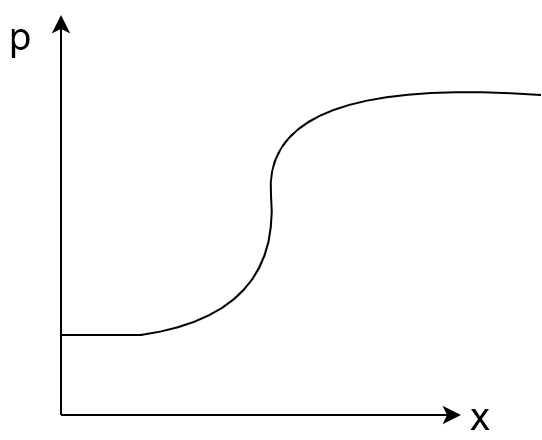
\includegraphics[scale=.7]{original.jpg} 
     \caption{元画像}
     \label{fig:original}
    \end{figure}
    図\ref{fig:original}の画像を一階微分した濃度変化を図\ref{fig:1calc}に示す。さらに二階微分した濃度変化を図\ref{fig:2calc}に示す。
    \begin{figure}[H]
     \centering
     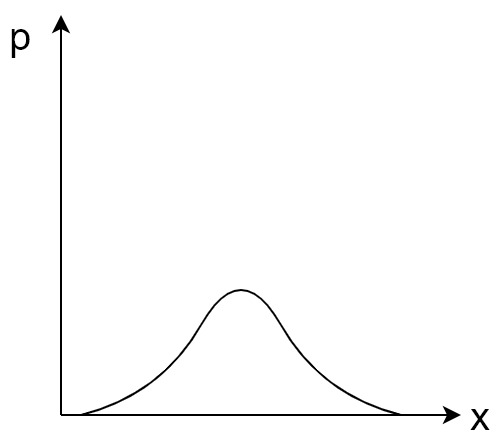
\includegraphics[scale=.7]{1calc.jpg} 
     \caption{一階微分}
     \label{fig:1calc}
    \end{figure}
    \begin{figure}[H]
     \centering
     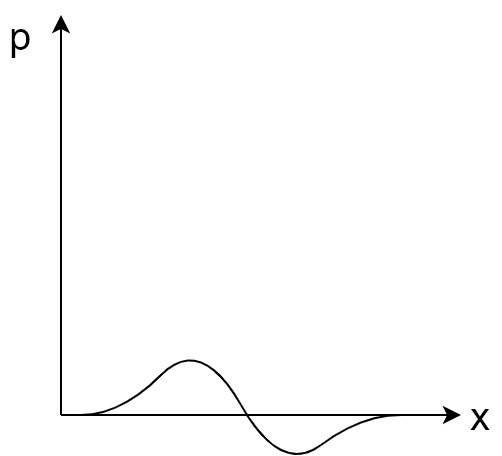
\includegraphics[scale=.7]{2calc.jpg} 
     \caption{二階微分}
     \label{fig:2calc}
    \end{figure}

    図\ref{fig:2calc}のように二階微分をすることで元画像の濃度変化する部分が出現することがわかる。
    画像データでは濃度変化は離散的に起こるため微分は単なる差分として表現することができる。
    式\eqref{eq:calcx},\eqref{eq:calcy}にそれぞれx方向、y方向の一階微分を示す。式\eqref{eq:calcx},\eqref{eq:calcy}にそれぞれ右上がり斜め方向、左上がり斜め方向の一階微分を示す。
    $i,j$は画像でのピクセルの存在する座標を示す。
    \begin{equation}\label{eq:calcx}
      f_x(i, j) = f(i + 1, j) - f(i, j)   
    \end{equation}
    \begin{equation}\label{eq:calcy}
      f_y(i, j) = f(i, j + 1) - f(i, j)   
    \end{equation}
    \begin{equation}\label{eq:calcr}
      f_r(i, j) = f(i + 1, j + 1) - f(i, j)   
    \end{equation}
    \begin{equation}\label{eq:calcl}
      f_l(i, j) = f(i - 1, j + 1) - f(i, j)   
    \end{equation}
    さらに微分した2階微分は式\eqref{eq:calcxx}--\eqref{eq:calcll}のようになる。
    \begin{equation}\label{eq:calcxx}
      f_{xx}(i, j) = \{f(i + 1, j) - f(i, j)\} - \{f(i, j) - f(i - 1,j)\}  
    \end{equation}
    \begin{equation}\label{eq:calcyy}
      f_{yy}(i, j) = \{f(i, j + 1) - f(i, j)\} - \{f(i, j) - f(i, j - 1)\}  
    \end{equation}
    \begin{equation}\label{eq:calcrr}
      f_{rr}(i, j) = \{f(i + 1, j + 1) - f(i, j)\} - \{f(i, j) - f(i - 1, j - 1)\}  
    \end{equation}
    \begin{equation}\label{eq:calcll}
      f_{ll}(i, j) = \{f(i + 1, j - 1) - f(i, j)\} - \{f(i, j) - f(i + 1, j - 1)\}  
    \end{equation}

    ここでラプラシアン$\nabla^2f(i,j)$を式\eqref{eq:laplacian}のように定義する.
    \begin{eqnarray}\label{eq:laplacian}
      \nabla^2f(i, j) &=& f_{ll}(i, j) + f_{yy}(i, j) +f_{rr}(i, j) +f_{ll}(i, j) \nonumber \\
      &=& f(i - 1, j- 1)  + f(i, j - 1) + f(i + 1, j - 1) + f(i - 1, j) + f(i + 1, j) + \nonumber\\
      &&f(i - 1, j + 1) + f(i, j + 1) + f(i + 1, j + 1) - 8f(i,j)
    \end{eqnarray}

    よって8近傍ラプラシアンフィルタを次のようになる。
    \begin{table}[H]
      \centering
      \begin{tabular}{|c|c|c|}
      \hline
      1 & 1  & 1 \\\hline
      1 & -8 & 1 \\\hline
      1 & 1  & 1 \\\hline
      \end{tabular}
    \end{table}

  \subsection{プログラム}
    プログラムリスト\ref{p:Filter-Laplacian}に空間フィルタによりラプラシアン8近傍を適用するプログラムを示す。
    \lstinputlisting[caption=ラプラシアン,label=p:Filter-Laplacian]{../Filter-Laplacian.c}

    コマンドライン引数として入出力ファイル、画像サイズとなるsizeを指定する。本プログラムでは画像の画素データを保持しておく必要があるため二次元配列を用いて各ピクセルの画素値を
    保存する。その際mallocによって領域を確保する.その後各ピクセルとその近傍8つのピクセルにマスクを適用し、その積和を変換後のピクセルの画素値としてputc関数にて出力バッファに書き込む。
    このとき積和が0以下であれば0として出力する。また255以上であれば255として出力する。
  
  \subsection{結果}
    図\ref{fig:building-lap},\ref{fig:after-building-lap}にラプラシアン8近傍の空間フィルタを適用する画像と適用した画像を示す。
    \begin{figure}[H]
      \centering
      \includegraphics[scale=.8]{./building.bmp}
      \caption{元画像}
      \label{fig:building-lap}
    \end{figure} 
    \begin{figure}[H]
      \centering
      \includegraphics[scale=.8]{./laplacian-building.bmp}
      \caption{空間フィルタ適用後の画像}
      \label{fig:after-building-lap}
    \end{figure}  
  
  \subsection{考察}
    図\ref{fig:building-lap},\ref{fig:after-building-lap}よりラプラシアン8近傍の空間フィルタを適用することでエッジ部分が白くなっていることがわかる。

\section{課題2(2)}
  本章では課題2(2)について課題内容、結果およびプログラムを示す。
  \subsection{課題内容}
    次に課題内容を示す.
    \begin{itembox}[l]{課題2(2)}
      画像の先鋭化を行うプログラムを示せ。
    \end{itembox}
  \subsection{理論}
    先鋭化とは元画像からラプラシアン画像を引くことである。
    図\ref{fig:diff}に二階微分した画像を元画像から引いた画像を示す。
    \begin{figure}[H]
     \centering
     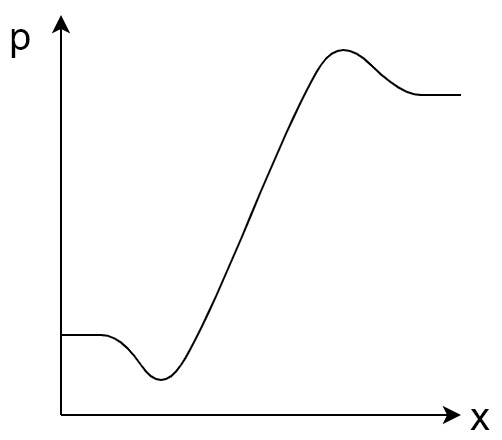
\includegraphics[scale=.7]{diff.jpg} 
     \caption{元画像-二階微分}
     \label{fig:diff}
    \end{figure}
    図\ref{fig:diff}より濃度変化が起こるエッジ部分を強調する画像を生成することができる。
    二階微分はラプラシアンとして式\ref{eq:laplacian}として定義したため、元画像から二階微分を引く先鋭化は式のように示される。
    \begin{eqnarray}\label{eq:sharp}
      g(i, j) &=& f(i ,j) - \nabla^2f(i,j) \nonumber\\
            &=& 9f(i,j) - f(i - 1, j- 1)  - f(i, j - 1) - f(i + 1, j - 1) - f(i - 1, j) -  \nonumber\\
            &&f(i + 1, j) - f(i - 1, j + 1) - f(i, j + 1) - f(i + 1, j + 1)  
    \end{eqnarray}

    よって先鋭化フィルタを次のようになる。
    \begin{table}[H]
      \centering
      \begin{tabular}{|c|c|c|}
      \hline
      -1 & -1  & -1 \\\hline
      -1 & 9 & -1 \\\hline
      -1 & -1  & -1 \\\hline
      \end{tabular}
    \end{table}
  \subsection{プログラム}
    プログラムリスト\ref{p:Filter-Laplacian}に空間フィルタにより先鋭化を行うプログラムを示す。
    \lstinputlisting[caption=先鋭化,label=p:Filter-Sharpening]{../Filter-Sharpening.c}

    コマンドライン引数として入出力ファイル、画像サイズとなるsizeを指定する。本プログラムでは画像の画素データを保持しておく必要があるため二次元配列を用いて各ピクセルの画素値を
    保存する。その際mallocによって領域を確保する.その後各ピクセルとその近傍8つのピクセルにマスクを適用し、その積和を変換後のピクセルの画素値としてputc関数にて出力バッファに書き込む。
    このとき積和が0以下であれば0として出力する。また255以上であれば255として出力する。
  
  \subsection{結果}
    図\ref{fig:building-sharp},\ref{fig:after-building-sharp}にラプラシアン8近傍の空間フィルタを適用する画像と適用した画像を示す。
    \begin{figure}[H]
      \centering
      \includegraphics[scale=.8]{./building.bmp}
      \caption{元画像}
      \label{fig:building-sharp}
    \end{figure} 
    \begin{figure}[H]
      \centering
      \includegraphics[scale=.8]{./sharp-building.bmp}
      \caption{空間フィルタ適用後の画像}
      \label{fig:after-building-sharp}
    \end{figure}  
  
  \subsection{考察}
    図\ref{fig:building-lap},\ref{fig:after-building-lap}より画像を先鋭化することでエッジ部分が鮮明に見えるようになった。

\section{課題2(3)}
  本章では課題2(3)について課題内容、結果およびプログラムを示す。
  \subsection{課題内容}
    次に課題内容を示す.
    \begin{itembox}[l]{課題2(2)}
      ラプラシアンの空間フィルタを適用した結果の画像を,適当な閾値を設定して2値化し,輪郭線画像を作成せよ.
    \end{itembox}
  \subsection{理論}
    式\eqref{eq:binarize}に二値化の変換関数を示す。thresholdは指定する閾値である。
    \begin{equation} \label{eq:binarize}
      f(x) = 
      \begin{cases}
      0   &   x < \text{threshold}  \\
      255        &  x > \text{threshold} 
      \end{cases}
    \end{equation} 
  \subsection{プログラム}
    プログラムリストに二値化プログラムを示す。
    \lstinputlisting[caption=二値化,label=p:binarize]{../binarize.c}
    コマンドライン引数として入出力ファイル、閾値となるthresholdを指定する。getc関数によって入力バッファから1バイトずつ読み取りint型変数cに格納する。
    putc関数により出力バッファに書き込む。このとき式\eqref{eq:binarize}を基に三項演算子によって場合分けを行う。
  \subsection{結果}
    図\ref{fig:building-binarize},\ref{fig:after-building-binarize}にそれぞれ輝度調整を行う画像、輝度調整を行った画像を示す。threshold=160である。

    \begin{figure}[H]
      \centering
      \includegraphics[scale=.8]{./laplacian-building.bmp}
      \caption{元画像}
      \label{fig:building-binarize}
    \end{figure} 
    \begin{figure}[H]
      \centering
      \includegraphics[scale=.8]{./binarize-building.bmp}
      \caption{二値化後の画像}
      \label{fig:after-building-binarize}
    \end{figure} 
  
  \subsection{考察}
   図\ref{fig:building-binarize},\ref{fig:after-building-binarize}より閾値を160にすることで輪郭線画像を作成することができた。
\end{document}